

\documentclass[16pt]{article}
\usepackage{graphicx}
\usepackage{array}
\usepackage[hidelinks]{hyperref}
\usepackage{color}

\begin{document}



\begin{titlepage}
 
   

       \hfill\hfill\hfill
\begin{figure}
	 \begin{center}  
	
\includegraphics[width=0.99\textwidth]{images/eyantralogo.png}
	 \end{center} 
\end{figure}

      \qquad {\LARGE{\textbf{e-Yantra Summer Internship-2015 \\ }}}
       
       \vspace{0.5cm}
       \qquad{\Large{\textbf{IoT Connected valves for irrigation of}}} \\  
       % Print the main header
      
       
       \qquad\qquad {\Large{\textbf{\hspace{3.2cm} greenhouse}}}\\ \\ \\ \\ \\ \\
        
       \qquad \qquad{\Large{\underline{\textbf{QUICK INSTALLATION GUIDE}}}}
         
  
          
\end{titlepage}
\tableofcontents
\vspace{15cm }

\section{Hardware}


\subsection{ESP8266 WiFi module}

\vspace{0.5cm}

ESP8266 is a low power WIFI module which is very much suitable for our
irrigation application. Some of the important features of the ESP8266
are:


\begin{itemize}

\item
  Its an ultra low power module which works on 3.3V. This is ideal for
  IoT applications
\item
  It has high on-chip integration
\item
  It has GPIO support for the application devices that you want to
  control
\item
  It has a 32 bit CPU
\item
  It is very small in size
\item
  It is a low cost module
\item
  It can act as a standalone device without the need of any external
  controller
\end{itemize}


\vspace{0.4cm}

We chose to go with ESP8266 over CC3200 because the ESP module had all
the functionalities that we needed and was cheaper, lighter and better
for IoT applications.




\subsection{IDE for ESP8266}

\begin{enumerate}

\item
  ESP8266 comes with the NodeMCU firmware loaded and it accepts LUA
  script which can be loaded into the board using ESplorer IDE, but the
  use of this IDE lacks proper documentation.
\item
  Download ESplorer from the website {\color{red}\href{http://esp8266.ru/esplorer/#download}{ESPlorer}}
\item
  LUA is an embeddable, fast, powerful and light script. This is useful in data
  description and has procedural syntax. It also has some other
  important features like: Automatic memory management and Garbage
  collection. Here's {\color{red}\href{http://www.lua.org/manual/5.3/}{LUA API}}
\item
  One other way of loading code into the ESP is using the Arduino
  IDE.This directly loads code into the EEPROM and the NodeMCU firmware
  can be loaded back in the ESP if
  needed. {\color{red}\href{https://learn.adafruit.com/adafruit-huzzah-esp8266-breakout/using-arduino-ide}{Using arduino}}
\item Clone arduino IDE fro ESP-Arduino Github repository and follow
  the installation procedure. {\color{red}\href{https://github.com/esp8266/Arduino.git}{Arduino}}. \textbf{But we prefer to inbuilt nodeMCU with ESPlorer IDE.}
\end{enumerate}



\subsection{Installation procedure:}

\begin{itemize}

\item
  Download nodeMCU latest firmware from the link above 
\item
  Download ESPTOOL
\item
  Move to the directory containing esptool and execute the following
  command
\end{itemize}

\begin{quote}
\texttt{sudo python esptool.py -{}-port /dev/ttyUSB0  write\_flash 0x00000 The\_Path\_To\_The\_NodeMCU\_Firmware.bin}
\end{quote}

\begin{itemize}

\item
  Make sure you are connected to the right port and change can access
  it. Else change ownership using
\end{itemize}

\begin{quote}
\texttt{Sudo chown \$username /dev/ttyUSB*}
\end{quote}

\textbf{note:} Make sure GPIO 0 is connected to ground while flashing
\vspace{0.5cm}

\subsection{ESPlorer IDE}

\begin{itemize}

\item
  The ESPlorer IDE is a great tool to work with the ESP8266 making the
  loading of code into the ESP an easy task
\item
  Download ESPlorer here
 {\color{red}\href{http://esp8266.ru/esplorer/\#download}{ESPlorer}}
\item
  ESPlorer is a platform that helps you load lua scripts into the ESP.
  follow this for more help
  {\color{red}\href{http://randomnerdtutorials.com/esp8266-web-server/}{webserver\_example}}
\item
  For the GPIO mapping refer this
  {\color{red}\href{https://github.com/nodemcu/nodemcu-firmware}{gpio\_map}}
\item
  Refer this for some more documentation regarding nodeMCU
  {\color{red}\href{http://www.nodemcu.com/docs/}{nodeMCU}}
\end{itemize}

\subsection{Troubleshooting}

\begin{itemize}

\item
  ESPlorer needs JAVA 7 or higher. install JAVA 8 for ubuntu by
  following these steps
  {\color{red}\href{http://tecadmin.net/install-oracle-java-8-jdk-8-ubuntu-via-ppa/}{JAVA 8}}.
  After downloading ESPlorer make your way to the folder in which
  ESPlorer.jar exists and run this command in the terminal
  \textgreater{}\texttt{java -jar ESPlorer.jar} and your done
\item
  esptool depends on {\color{red}\href{http://pyserial.sourceforge.net/}{pySerial}}
  for serial communication with the target device.
\end{itemize}

If you choose to install esptool system-wide by running
\texttt{python setup.py install}, then this will be taken care of
automatically.
If not using \texttt{setup.py}, then you'll have to install pySerial
manually by running something like \\

\texttt{pip install pyserial},
\texttt{easy\_install pyserial} or
\texttt{apt-get install python-serial} \\
\vspace{0.3cm}
depending on your platform. The
official pySerial installation instructions are
{\color{red}\href{http://pyserial.sourceforge.net/pyserial.html\#installation}{here}}).
This utility actually have a user interface! It uses
{\color{red}\href{https://docs.python.org/dev/library/argparse.html}{Argparse}}
and is rather self-documenting. Try running \texttt{esptool -h}. Or hack the
script to your hearts content. The serial port is selected using the
\texttt{-p} option, like \texttt{-p /dev/ttyUSB0} (on unixen like Linux
and OSX) or \texttt{-p COM1} (on Windows). The perhaps not so obvious
corner case here is when you run esptool in Cygwin on Windows, where you
have to convert the Windows-style name into an Unix-style path
(\texttt{COM1} -\textgreater{} \texttt{/dev/ttyS0}, and so on).

\vspace{19cm}

\section{Server Installation}
 
\vspace{1cm}                                    % Print the main header


 
\subsection{Ubuntu}

\hfill
  \begin{enumerate}
  \item
    Have Ubuntu image in pen-drive or a cd
  \item
    Take care to disable secure boot before installation
  \item
    After installation if windows doesn't show in the boot options then
    repair the GRUB from UBUNTU using \emph{boot repair}.Have boot repair in a disc or pen-drive.
  \item
    If you use face further problems use GRUB customizer from UBUNTU.Install Grub customizer from software centre.
  \item
    Once Windows shows in boot options then change the Boot preference
    order from windows by going to the bios setup.
  \item
    In Sony systems while booting use \emph{ASSIST} key
  \end{enumerate}
  
for further information look up \\

{\color{red}\href{https://help.ubuntu.com/community/WindowsDualBoot}{Ubuntu Insatllation}}
  
\hfill


\subsection{Installation of Apache2, PHP and MySQL (LAMP-server)}

\vspace{0.5cm}

{\underline{\Large{About LAMP}}}

  LAMP stack is a group of open source software used to get web servers up
  and running. The acronym stands for Linux, Apache, MySQL, and PHP. Since
  the virtual private server is already running Ubuntu/openSuse, the linux
  part is taken care of. Here is how to install the rest.


  
  

  
%  \begin{center}\rule{3in}{0.4pt}\end{center}

  \subsubsection{Install Apache}
  
  \hfill

  To install apache, open terminal and type in these commands: \\
  \textbf{For Ubuntu} \\
  \texttt{sudo apt-get update} 

  \texttt{sudo apt-get install apache2}

  \textbf{For openSuse}

  \texttt{sudo zypper in apache2}

  \textbf{Firewall Adjustments}

  In openSuse, by default the firewall configuration blocks all traffic
  coming on port 80 to your machine. So if you need to allow access so
  that the web server can be accessed from within a LAN we need to fine
  tune the firewall configuration. The below step needs to be performed as
  root user. The supplied configurations are called apache2 and
  apache2-ssl. They can be enabled via YaST, by adding them to
  FW\_CONFIGURATIONS\_EXT in the following path /etc/sysconfig/SuSEfirewall2
  
  \vspace{0.5cm}

  \texttt{sysconf\_addword /etc/sysconfig/SuSEfirewall2 FW\_CONFIGURATIONS\_EXT apache2}
  \texttt{sysconf\_addword /etc/sysconfig/SuSEfirewall2 FW\_CONFIGURATIONS\_EXT apache2-ssl}
  \texttt{rcSuSEfirewall2 restart}
  
   \vspace{0.5cm}

  \textbf{Starting Server}

  Start the server and configure it to automatically start at boot time.

  \texttt{rcapache2 start} \texttt{chkconfig -a apache2}
  
   \vspace{0.5cm}

  \subsubsection{Install MySQL}
  
   \vspace{0.5cm}

  MySQL is a powerful database management system used for organizing and
  retrieving data

  To install MySQL, open terminal and type in these commands:

  \textbf{For Ubuntu} \\ sudo apt-get install mysql-server
  libapache2-mod-auth-mysql php5-mysql

  \textbf{For openSuse}

  \texttt{sudo zypper install mysql-server}

  \textbf{To start the server}

  \texttt{sudo systemctl start mysql.service}
  
   \vspace{1cm}

  \subsubsection{Install PHP}
   \vspace{0.5cm}

  PHP is an open source web scripting language that is widely use to build
  dynamic webpages.

  To install PHP, open terminal and type in this command.

  \textbf{For Ubuntu}

  \texttt{sudo apt-get install php5 libapache2-mod-php5 php5-mcrypt}

  \textbf{For openSuse}

  \texttt{sudo zypper in php5 php5-mysql apache2-mod\_php5}
  
   \vspace{0.5cm}

  {\underline{\textbf{Installing phpMyAdmin}}}

  \textbf{For Ubuntu}

  \texttt{sudo apt-get install phpMyAdmin}

  \textbf{For OpenSuse}

  \texttt{sudo zypper in phpMyAdmin}
   \vspace{0.5cm}

  Finally restart apache so that all of the changes take effect:

  \textbf{For Ubuntu}

  \texttt{sudo service apache2 restart}

  \textbf{For openSuse}

  \texttt{sudo systemctl start apache2.service}
   \vspace{0.5cm}

 

  



\vspace{13cm}

\section{MOSCA broker}

\vspace{0.5cm}
\subsection{Broker and nodejs}

\vspace{0.5cm}

Based on their use, there are two widely available MQTT brokers
available on the web.
\begin{enumerate}
	{\color{red}{\item\href{http://mosquitto.org/}{Mosquitto}}} 
	{\color{red}{\item\href{https://github.com/mcollina/mosca}{Mosca}}}
\end{enumerate}
We chose Mosca because it is: 

\begin{enumerate}
	
	\item MQTT 3.1 compliant.
	\item supporting various storage options for QoS 1 offline packets, and subscriptions.
	\item As fast as it is possible.
	\item Usable inside ANY other Node.js app.
	
\end{enumerate}
\vspace{0.5cm}




\textbf{Installation on a OpenSuse system (version
	13.1)}

\textbf{Part 1} First install nodejs and npm if both are absent in your
system.


\textbf{Nodejs}

\begin{quote}
	\texttt{sudo zypper install nodejs}
\end{quote}

\textbf{npm}

\begin{quote}
	\texttt{sudo zypper install npm}
\end{quote}

If everything goes right (no errors) then proceed to second part.
\vspace{0.5cm}

\textbf{Part 2}

\textbf{Installation of Mosca}

\begin{quote}
	\texttt{npm install Mosca}
\end{quote}

If everything goes write then you are good to go.
\vspace{0.5cm}

\textbf{To start the broker} \textgreater{}\texttt{mosca -v --host yourhostipaddress |bunyan}


\textbf{Installation on an Ubuntu system (version
	14.4)}

\textbf{Part 1} First install nodejs and npm if both are absent in your
system.

\textbf{Nodejs}

\begin{quote}
	\texttt{sudo apt-get update}
\end{quote}

\begin{quote}
	\texttt{sudo apt-get install nodejs}
\end{quote}

\begin{quote}
	\texttt{sudo ln -s /usr/bin/nodejs /usr/bin/node}
\end{quote}

\textbf{npm}

\begin{quote}
	\texttt{sudo apt-get install npm}
\end{quote}

If everything goes right (no errors) then proceed to second part.

\vspace{0.3cm}

\textbf{Part 2}

\textbf{Installation of Mosca}

\begin{quote}
	\texttt{sudo npm install debug}
\end{quote}

\begin{quote}
	\texttt{sudo npm install mosca bunyan -g} //for installing mosca
	globally
\end{quote}

\begin{quote}
	\texttt{sudo npm install daemon}
\end{quote}



If everything goes write then you are good to go.

\vspace{0.3cm}

\textbf{To start the broker} \textgreater{}\texttt{mosca -v --host yourhostipaddress |bunyan}



\vspace{0.5cm}

\subsection{Testing the broker}

First to test the mqtt broker, we need to install a mqtt client on the
system.

\begin{quote}
	\texttt{sudo npm install mqtt -g}
\end{quote}

\textbf{Second, creating scripts for testing}

Script for starting MQTT broker service, \textbf{mosca-app.js}

To start the service type \textgreater{}\texttt{node mosca-app.js}

\vspace{0.5cm}
Script for publishing, \textbf{client-pub.js}

Open a new Terminal and Execute above MQTT Subscription Client
client-sub.js \textgreater{}\texttt{node client-pub.js}

\vspace{0.5cm}
Script for subscribing, \textbf{client-sub.js}

Now open a differnent Terminal and Execute above MQTT Subscription
Client client-pub.js \textgreater{}\texttt{node client-sub.js}

\vspace{0.5cm}
\textbf{Successful Output From client-sub.js terminal}

\begin{quote}
	\texttt{Hello!}
\end{quote}


\begin{figure}
	\hspace{2cm}
	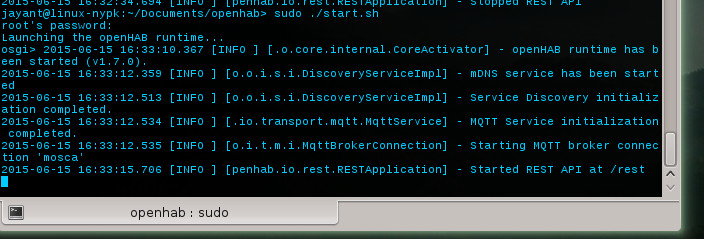
\includegraphics[width=0.7\textwidth]{images/mosca.jpg}
	\caption{MOSCA start}
\end{figure}

\vspace{0.5cm}

\subsection{Troubleshooting}

%\begin{center}\rule{3in}{0.4pt}\end{center}

If while installing mosca there are errors in fetching the links from
server, do any of the following 

\begin{itemize}
	
	\item Check that nodejs version is not
	`pre', if it is then update it to a stable non pre version.
	\item reinstalling nodejs and npm in root mode. 
	\item restart your system.
	
\end{itemize}

While executing those scripts, if any of the nodejs script file shows
error \textbf{Mqtt module not found}, then copy the scripts to a folder
inside mosca directory, and try executing from there.

For \textbf{openSuse} users, open firewall in yast2 GUI. Then go to
allowed service, then go to to advance option, there enter 1883 inside
tcp port.

After successfully installing MOSCA broker on the system, you are now
good to go on next step.

\vspace{0.5cm}
\subsection{Running MOSCA}

\vspace{0.3cm}



\subsubsection{Configuring IP on which MOSCA has to be run.}

\emph{on the terminal type \textgreater{}\texttt{mosca -help}, it will
display all the handles which mosca currently supports we are going to
use handles, {\textbf{-v, --host, \textbar{} bunyan}}}. \emph{To start the server,on
the terminal type \textgreater{}\texttt{mosca -v --host 'ur ip'
\textbar{}bunyan}}. \\ Server testing can be done via two codes included in
the software folder.

 

\vspace{0.3cm}

\textbf{NOTE}: for openSUSE users, make sure that entry for tcp port
1883 is in the firewall for inbound connection.

\begin{itemize}

\item
  to run the code, first run client-sub.js on a different terminal, and
  then run client-pub.js on a second terminal.
\item
  message from the topic subscribed will be printed where client-sub.js
  has been run.
\end{itemize}



\vspace{0.5cm}

\subsubsection{Interfacing MOSCA and ESP}

\begin{itemize}

\item
  Install MOSCA on your system
\item
  Setup the server using \emph{mosca -v --host \$hostname \textbar{}
  bunyan}
\item
  Burn the LUA scripts on the ESP8266
\item


  send subscribe request from your terminal using
  \textgreater{}\texttt{node client-sub.js} (go to the apprpriate folder
  first)
\item
  send publish command from the terminal
  \textgreater{}\texttt{node client-pub.js}
\item
  see the sent data on your terminal with confirm message
\end{itemize}



\subsection{Troubleshooting}


\subsubsection{ESP8266}

\begin{itemize}

\item
  take care to use the delays at appropriate places so as to send out
  publish and subscribe requests
\item
  LUA syntax must be kept in mind.
\item
  Use \textgreater{}\texttt{tmr.alarm} instead of
  \textgreater{}\texttt{tmr.delay} wherever possible
\end{itemize}

\vspace{0.6cm}

\subsubsection{MOSCA server}

\begin{itemize}

\item
  The local IP must be changed in the the ESP and also the
  \textgreater{}\texttt{client-pub.js} and
  \textgreater{}\texttt{client-sub.js} scrits
\item
  The topic must be the same in the \textgreater{}\texttt{client-pub.js}
  and subscribe code in the ESP
\end{itemize}

\vspace{0.5cm}



\vspace{12cm}

\section{Setting up the website}
{{\textbf{UI part consist of PHP core, MySQL and phpMQTT library(SSKAJE) }}}
\subsection{Database}
\vspace{0.3cm}
{\Large{\underline{\textbf{Table Description}}}}
\vspace{0.2cm}
Create database named 'iot', and above tables with below mentioned format.\\
\textbf{Database name: iot}

Tables in database: 

\begin{itemize}

\item devices
\item groups 
\item sensors
\item tasks  

\end{itemize}

\textbf{Device table}

\textbf{Name:} Devices

\begin{quote}

	\centering
	 \caption{Table 1: Devices table}
	\label{my-label}
	\begin{tabular}{llllll}
		{\bf FIELD} & {\bf TYPE}   & {\bf NULL} & {\bf KEY} & {\bf Default}      & {\bf EXTRA}     \\
		id          & int(255)     & NO         & PRI       & NULL               & auto\_increment \\
		name        & varchar(255) & YES        &           & NULL               &                 \\
		macid       & varchar(30)  & NO         &           & NULL               &                 \\
		group       & varchar(255) & YES        &           & NULL               &                 \\
		status      & int(1)       & YES        &           & NULL               &                 \\
		battery     & int(1)       & YES        &           & NULL               &                 \\
		timestamp   &              & NO         &           & CURRENT\_TIMESTAMP &                 \\
		action      & varchar(255) & YES        &           & NULL               &                
	\end{tabular}
	
\end{quote}
\textbf{Group Table}

\textbf{Name:} groups

\begin{quote}
	\centering
	\caption{Table 2: Groups table}
	\label{my-label}
	\begin{tabular}{llllll}
		{\bf FIELD} & {\bf TYPE}   & {\bf NULL} & {\bf KEY} & {\bf Default} & {\bf EXTRA}     \\
		id          & int(10)      & NO         & PRI       & NULL          & auto\_increment \\
		name        & varchar(255) & NO         &           & NULL          &                
	\end{tabular}

\end{quote}
\textbf{Sensor Table}

\textbf{Name:} sensors

\begin{quote}
	\centering
	\caption{Table 3: Sensors Table}
	\label{my-label}
	\begin{tabular}{llllll}
		{\bf FIELD} & {\bf TYPE}   & {\bf NULL} & {\bf KEY} & {\bf Default} & {\bf EXTRA}     \\
		id          & int(10)      & NO         & PRI       & NULL          & auto\_increment \\
		name        & varchar(255) & NO         &           & NULL          &                
	\end{tabular}

\end{quote}
\textbf{Tasks Table}

\textbf{Name:} tasks
\begin{quote}
\centering
\caption{Table 4: Tasks Table}
\label{my-label}
\begin{tabular}{llllll}
	{\bf FIELD} & {\bf TYPE}   & {\bf NULL} & {\bf KEY} & {\bf Default} & {\bf EXTRA}     \\
	id          & int(10)      & NO         & PRI       &           & auto\_increment \\
	item        & varchar(255) & NO         &           & NULL          &                 \\
	start       & int(4)       & YES        &           & NULL          &                 \\
	stop        & int(4)       & YES        &           & NULL          &                 \\
	action      & int(1)       & YES        &           &               &                
\end{tabular}
\end{quote}






\subsection{PHP core}

After setting up the database and its tables, copy IOT folder inside Software folder of the repo to your htdocs folder(linux).
There are few files which needs to be run in background for data gathering, such as device discovvery, battery status and moisture value.

\begin{enumerate}

\item Device discovery \textbf{--\textgreater{}}
\texttt{subscribe.php}
\item Valve and other sensors scheduling
\textbf{--\textgreater{}} \texttt{tasks.php} 
\item Listening for battery status \textbf{--\textgreater{}} \texttt{battery.php} 
\item Listening for Moisture value \textbf{--\textgreater{}} \texttt{moisture.php}

\end{enumerate}


Tasks.php is executed every minute using cron and above other files are
run continuously in php cli mode.

To use cron feature for tasks.php, go to terminal and type\\
\texttt{* * * * * /usr/bin/php destinationtoabovephpfiles/tasks.php}\\

To use cli mode, go to terminal and type

\texttt{/usr/bin/php destinationtoabovephpfiles}\\

\textbf{Main php files are:}\\
\texttt{index.php}-for managinng the manual control of the sensors\\
\texttt{devdis.php}-for seeing devices\'  status and other values including battery status}\\
\texttt{time.php}{-for scheduling automated tasks}\\
\texttt{manage.php}-for adding types of sensors, groups and newly discovered devices}\\\\
\textbf{MQTT Library used}

Uses php library \textbf{SSKAJE MQTT} for communicating with MOSCA
broker.

{\color{red}\href{https://sskaje.me}{SSKAJE MQTT}}

{\color{red}\href{https://github.com/sskaje/mqtt}{GITHUB}}\\
\textbf{About the website/Screenshots}



\vspace{5cm}

\end{document}